\documentclass{beamer}

\usepackage{amsmath}
\usepackage{amssymb}

\begin{document}
	%======================================================= % 
	%	\item Measuring risk in a micro dataset is a key task. Risk measurements are essential
	%	to determine if the dataset is secure enough to be released. To assess disclosure
	%	risk, one must make realistic assumptions about the information data users might
	%	have at hand to match against the micro dataset, these assumptions are called
	%	disclosure risk scenarios. 
	%	
	%	\item This goes hand in hand with the selection of categorical
	%	key variables because the choice these identifying variables defines a specific dis-
	%	closure risk scenario. 
	%	\item The specific set of chosen key variables has direct influence
	%	on the risk assessment because their distribution is a key input for the calculation
	%	of both individual and global risk measures as it is now discussed.
	%------------------------------------------------------------------------------%
\begin{frame}	
\frametitle{Measuring Risk}
\begin{itemize}
\item Measuring risk in a micro dataset is a key task. Risk measurements are essential
	to determine if the dataset is secure enough to be released. 
\item To assess disclosure
	risk, one must make realistic assumptions about the information data users might
	have at hand to match against the micro dataset; these assumptions are called
	disclosure risk scenarios. 
\item This goes hand in hand with the selection of categorical
	key variables because the choice these identifying variables defines a specific disclosure risk scenario. 
\end{itemize}
\end{frame}
%\begin{frame}	
%	\frametitle{Measuring Risk}
%	\begin{itemize}
%		\item The specific set of chosen key variables has direct influence on
%	the risk assessment because their distribution is a key input for the estimation of
%	both individual and global risk measures as it is now discussed. \item For example, for a
%	disclosure scenario for the European Union Structure of Earnings Statistics we can
%	assume that information on company size, economic activity, age and earnings of
%	employees are available in available data bases. \item Based on a specific disclosure risk
%	scenario, it is necessary to define a set of key variables (i.e., identifying variables)
%	that can be used as input for the risk evaluation procedure.
%	% Usually different scenarios are considered. 
%\end{itemize}
%\end{frame}
%\begin{frame}	
%	\frametitle{Measuring Risk}
%	\begin{itemize}
%	
%	\item For example, for the European Union Structure of Earnings
%	Statistics a second scenario based on an additional key varibles is of interest to
%	look at. e.g. occupation might be considered  well as an categorical key variable.
%	\item The resulting risk might now be higher than for the previous scenario. It needs
%	discussion with subject matter specialists which scenario is most realistic and an
%	evaluation of different scenarios helps to get a broader picture about the disclosure
%	risk in the data.
%\end{itemize}
%\end{frame}
%---------------------------------------------------------------------------------%
\subsection*{Population Frequencies and the Individual Risk Appoach}
\begin{frame}	
	\frametitle{Population Frequencies}
	\begin{itemize}
		\item 
	\item Typically, risk evaluation is based on the concept of uniqueness in the sample
	and / or in the population. The focus is on individual units that possess rare com	binations of selected key variables.
	\item The assumption is that units having rare
	combinations of key variables can be more easily identified and thus have a higher
	risk of re-identification/disclosure. 
	\item It is possible to cross-tabulate all identifying
	variables and view their cast. 
	\item Keys possessed by only very few individuals are
	considered risky, especially if these observations also have small sampling weights.
	This means that the expected number of individuals with these patterns is expected to be low in the population as well.
\end{itemize}
\end{frame}
%% -- Page 6 / 31
%% 2 MEASURING THE DISCLOSURE RISK
\begin{frame}	
	\frametitle{Population Frequencies}

\begin{itemize}
	\item To assess whether a unit is at risk, a threshold approach is typically used. If the
	risk of re—identification for an individual is above a certain threshold value, the unit
	is said to be at risk. 
	\item To compute individual risks, it is necessary to estimate the
	frequency of a given key pattern in the population. 
	
	\item Let us define frequency counts
	in a mathematical notation. Consider a random sample of size n drawn from a
	finite population of size N. Let $\pi_j$, $j = 1, \ldots ,N$ be the (first order) inclusion
	probabilities — the probability that element $u_j$ of a population of the size N is
	chosen in a sample of size n.
\end{itemize}
\end{frame}

%----------------------------------------------------------------------------%
\begin{frame}	
	\frametitle{Population Frequencies}
	
\begin{itemize}
	\item All possible combinations of categories in the key variables (i.e., keys or patterns)
	can be calculated by cross-tabulation of these variables.
	\item Let $f_i$, $i=1,2,\ldots,n$ be
	the frequency counts obtained by cross-tabulation and let $F_i$ be the frequency
	counts of the population which belong to the same pattern. 
	\item If $f_i=1$ applies,
	the corresponding observation is unique in the sample given the key-variables. If
	\item If $F_i = 1$, then the observation is unique in the population  well and automatically
	unique or zero in the sample.
	%----------------------------------------------------------------------------%
	\item $F_i$ is usually not known, since, in statistics, information on samples is collected
	to make inferences about populations.
\end{itemize}
\end{frame}
\begin{frame}
	\begin{figure}
\centering
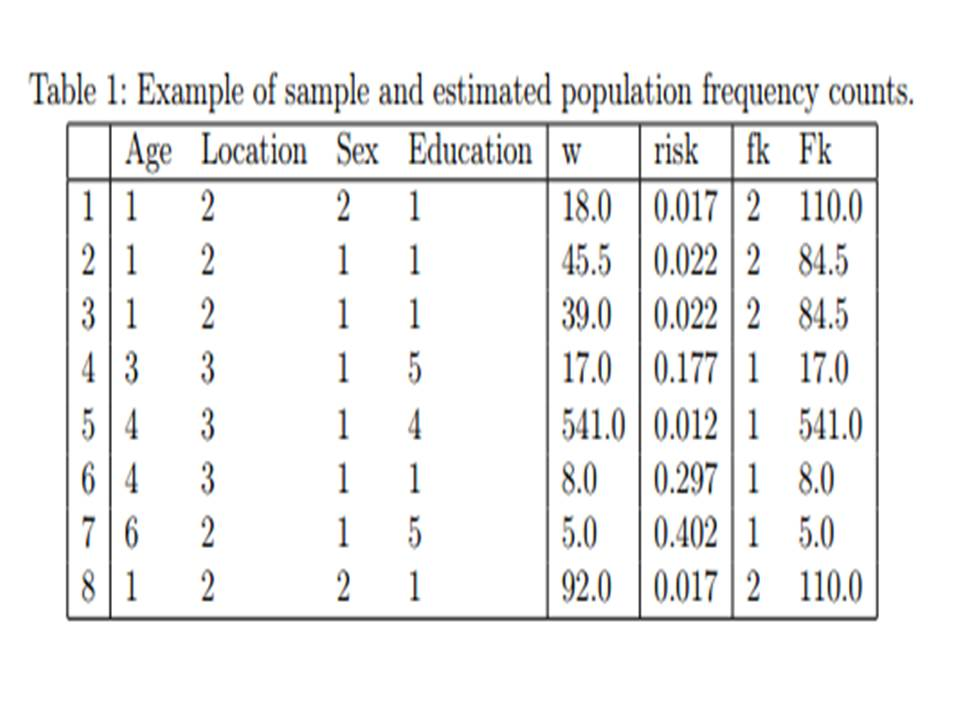
\includegraphics[width=0.9\linewidth]{JPEGS/TemplTable1}
\caption{}
\label{fig:TemplTable1}
\end{figure}

\end{frame}
	%----------------------------------------------------------------------------%
	\begin{frame}	
		\frametitle{Population Frequencies}
		
\begin{itemize}
	\item In Table 1 a very simple data set is used to explain the calulation of sample
	frequency counts and the (first rough) estimation of population frequency counts.
	One can easily see that observation 1 and 8 are equal, given the key-variables Age
	Class , Location, Sex and Education. Because the values of observations 1 and
	8 are equal and therefore the sample frequency counts are $f_1=2$ and $f_8=2$.
\end{itemize}
\end{frame}
%----------------------------------------------------------------------------%
\begin{frame}	
	\frametitle{Population Frequencies}
	
	\begin{itemize}
	\item Estimated population frequencies are obtained by summing up the sample weights
	for equal observations. 
	\item Population frequencies $\hat{F}_1$ and $\hat{F}_8$ can then be estimated
	by summation over the corresponding sampling weights, $w_1$ and $w_8$. 
	\item In summary,
	two observations with the pattern (key) (1,2,5, 1) exist in the sample and 110
	observations with this pattern (key) can be expected to exist in the population.
\end{itemize}
\end{frame}

	%----------------------------------------------------------------------------%
	\begin{frame}	
		\frametitle{Population Frequencies}
		
%----------------------------------------------------------------------------%
% % Graphic
% % Table 1: Example of sample and estimated population frequency counts.
% % TemplTable1.jpg

%----------------------------------------------------------------------------------------%
\end{frame}
	%----------------------------------------------------------------------------%
	\begin{frame}	
		\frametitle{Population Frequencies}
		
		\begin{itemize}
	\item One can show, however, that these estimates almost always overestimate small
	population frequency counts .
	%see, e.g., Templ and l\leill<ll, 2010].
	
	\item A better approach is to use so-called super—population models, in which population frequency
	counts are modeled given certain distributions. 
	
	\item For example, the estimation procedure of sample counts given the population counts can be modeled by assuming
	a negative binomial distribution and is implemented
	in \textbf{sdcMicro} in function \texttt{measurelisk()}
	and called by the
	\textbf{sdcMicroGUI}.
\end{itemize}	
\end{frame}
	%----------------------------------------------------------------------------%
	\begin{frame}	
		\frametitle{Population Frequencies}
		
\begin{figure}
\centering
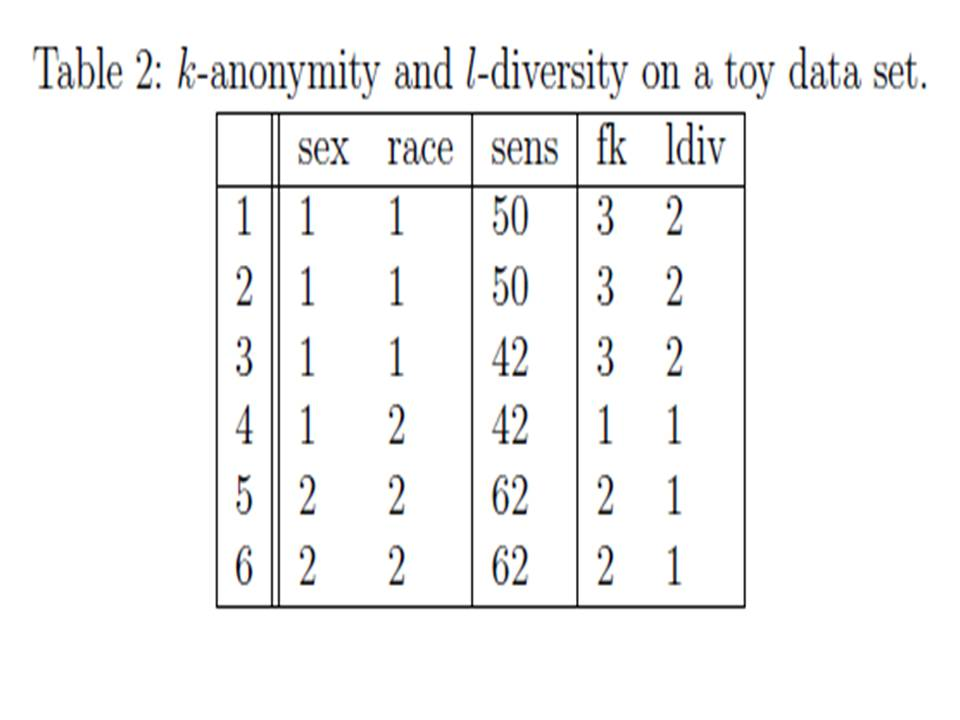
\includegraphics[width=0.99\linewidth]{TemplJPGs2/Table2}
\caption{}
\label{fig:Table2}
\end{figure}

%%Page 7 / 31
%--------------------------------------------------------------------

%2 MEASURING THE DISCLOSURE RISK
%Table 2: is-anonymity and l-diversity on a toy data set.
\end{frame}
\end{document}
		